\documentclass[norsk]{beamer}

\usepackage[utf8]{inputenc} % For æ, ø, å

\usepackage{babel}          % For oversettelser


\usetheme{MathDept}

\author{Fredrik Meyer}
\title{Singulariteter og singulære {personligheter}}
\subtitle{Algebraisk geometri for noobs}

\begin{document}
   
\section{Oversikt}

% Bruk 
%
%     \begin{frame}[allowframebreaks] 
%
% hvis innholdsfortegnelsen ikke får plass på ett lysark.

\begin{frame}
    \frametitle{Ordinær innholdsfortegnelse}
    \tableofcontents
\end{frame}

\begin{frame}
    \frametitle{Innholdsfortegnelse som fremhever nåværende seksjon}
    \tableofcontents[currentsection]
\end{frame}

\begin{frame}

  \begin{columns}[T]
    \begin{column}{.5\textwidth}
     \begin{block}{Node}
% Your text here
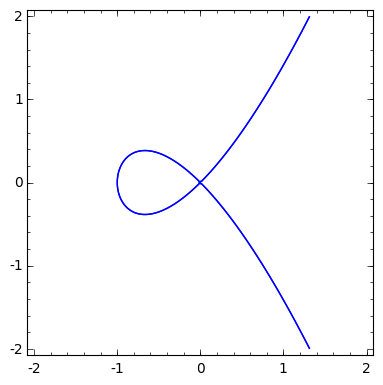
\includegraphics[scale=0.8]{presentasjon/node.png}
    \end{block}
    \end{column}
    \begin{column}{.5\textwidth}
    \begin{block}{Køsp}
% Your image included here

\includegraphics[scale=0.8]{presentasjon/cusp.png}
    \end{block}
    \end{column}
   \end{columns}


\end{frame}

\section{Algebraisk geometri}

\subsection{Teorem}

\begin{frame}
    \frametitle{Matematikk}

    \begin{theorem}[Fermats lille sats]
        For et primtall $p$ og $a \in \mathbb{Z}$ er $a^p \equiv a \pmod{p}$.
    \end{theorem}
    
    \begin{proof}
        De inverterbare elementene i en kropp danner en gruppe under multi\-plikasjon. Spesielt danner elementene 
        \[
            1, 2, \ldots, p-1 \in \mathbb{Z}_p
        \] 
        en gruppe under multiplikasjon modulo $p$. Denne gruppen har orden $p-1$. For $a \in \mathbb{Z}_p$ og $a \neq 0$ har vi dermed at $a^{p-1} = 1 \in \mathbb{Z}_p$. Setningen følger umiddelbart.
    \end{proof}   
\end{frame}

\subsection{Eksempel}

\begin{frame}
    \frametitle{Matematikk}
    
    \begin{example}
        Funksjonen $\phi \colon \mathbb{R} \to \mathbb{R}$ gitt ved $\phi(x) := 2x$ er kontinuerlig i punktet $x := \alpha$, fordi hvis $\epsilon > 0$ og $x \in \mathbb{R}$ er slik at $|x - \alpha| < \delta := \frac{\epsilon}{2}$, da er
        \begin{align*}
            |\phi(x) - \phi(\alpha)| = 2|x - \alpha| < 2\delta = \epsilon.
        \end{align*}
    \end{example}
\end{frame}

\section{Fremheving}

\begin{frame}
    \frametitle{Fremheving}
    
    Av og til er det nyttig å kunne \alert{utheve} enkelte ord midt i teksten.
    
    \begin{alertblock}{Viktig melding}     
        Hvis man har mye tekst som skal \alert{utheves} kan det være lurt å plassere den i en egen boks.
    \end{alertblock}
    
    Det er lett å få tekst til å passe \structure{fargetemaet}.
\end{frame}

\section{Lister}

\begin{frame}
    \frametitle{Lister}
    
    \begin{itemize}
        \item Punktlister markeres med en grå boks.
    \end{itemize}
    
    \begin{enumerate}
        \item Nummererte lister markeres med en større grå boks og hvitt nummer.
    \end{enumerate}
    
    \begin{description}
        \item[Beskrivelser] fremhever viktige begreper med grå tekst.
    \end{description}
    
    \begin{alertblock}{Alertblock}
        \begin{itemize}
            \item Lister skifter farge etter omgivelsene.
        \end{itemize}        
    \end{alertblock}
    
    \begin{example}
        \begin{itemize}
            \item Lister skifter farge etter omgivelsene.
        \end{itemize}        
    \end{example}
\end{frame}

\section{Referanser}

\begin{frame}[allowframebreaks]
    \frametitle{Referanser}    
    
    \begin{thebibliography}{}    

        % Article er forhåndsvalgt.
        \setbeamertemplate{bibliography item}[book] 
        
        \bibitem{Hartshorne1977}
        R.~Hartshorne.
        \newblock \emph{Algebraic Geometry}.
        \newblock Springer-Verlag, 1977.
       
        \setbeamertemplate{bibliography item}[article]
        
        \bibitem{Artin1966}
        M.~Artin.
        \newblock On isolated rational singularities of surfaces.
        \newblock \emph{Amer. J. Math.}, 80(1):129--136, 1966.  
       
       \setbeamertemplate{bibliography item}[online]
        
       \bibitem{Vakil2006}
       R.~Vakil.
       \newblock \emph{The moduli space of curves and Gromov-Witten theory}, 2006.
       \newblock \url{http://arxiv.org/abs/math/0602347}
       
       \setbeamertemplate{bibliography item}[triangle]
       
       \bibitem{AM1969}
       M.~Atiyah og I.~Macdonald.
       \newblock \emph{Introduction to commutative algebra}.
       \newblock Addison-Wesley Publishing Co., Reading, Mass.-London-Don
       Mills, Ont., 1969
           
       \setbeamertemplate{bibliography item}[text]
       
       \bibitem{Fraleigh1967}
       J.~Fraleigh.
       \newblock \emph{A first course in abstract algebra}.
       \newblock Addison-Wesley Publishing Co., Reading, Mass.-London-Don Mills, Ont., 1967
    \end{thebibliography}
\end{frame}

\end{document}









